\subsection{CentralControl IBD}

\begin{figure}[H]
	\centering
	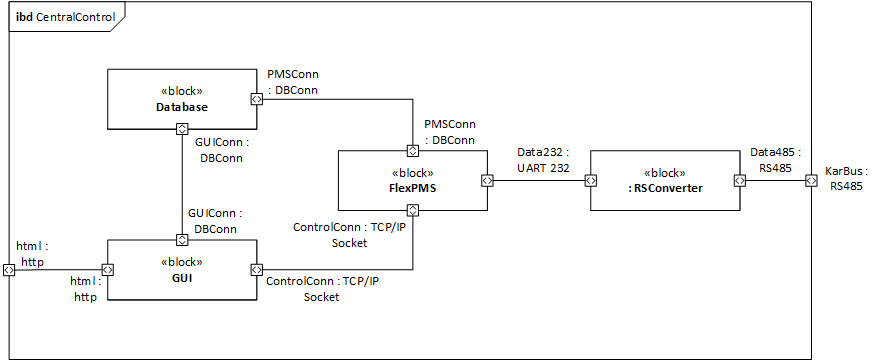
\includegraphics[width=0.82\textwidth]{Systemarkitektur/CentralStyring/CentralControl_IBD.png}
	\label{fig:CentralControl IBD}
	\caption{Internal Block Diagram af CentralControl}
\end{figure}

\subsection{Signal beskrivelser}

\begin{table}[H]
\centering
{\rowcolors{2}{white!80!black!30}{white!70!black!60} %farver på hver anden række -starter på 3
\setlength{\arrayrulewidth}{0.2mm}					 %tykkelse på linier 
\setlength{\tabcolsep}{10pt}						 %indryk i celle 
\renewcommand{\arraystretch}{1.5}					 %højden på tabelrum
\center
\begin{tabular}{|p{20mm}|p{40mm}|p{30mm}|p{30mm}|}		 %længden på alle rum
\hline

\multicolumn{4}{|>{\columncolor{white!20!black!90}}m{14.20cm}|}{\textcolor{white}{\large{\textbf{Signal beskrivelser}}}} \\\hline
\rowcolor{white!70!black!60}
\textcolor{black}{\large{\textbf{Navn}}}&
\textcolor{black}{\large{\textbf{Definition}}}&	
\textcolor{black}{\large{\textbf{Område}}}&
\textcolor{black}{\large{\textbf{Kommentar}}}\\
\hline
KarBus				& RS485 bus til kommunikation mellem enheder &	 	& Differentielt bussystem  \\
Data485				& RS485 bus til kommunikation mellem enheder &	 	& internt signal   \\
Data232				& RS485 konverteret til logisk niveau		 &	 	& Signal efter konvertering  \\
PMSConn				& Database forbindelse						 &		& Til at skrive log \\
GUIConn				& Database forbindelse						 &		& Til at hente og skrive indstillinger samt log \\
ControlConn			& Socket forbindelse fra GUI til FlexPMS	 &		& Til at sende kommandoer fra GUI til FlexPMS \\
html				& Http protokol								 &		& Fobindelse til brugerens browser \\
\hline
\end{tabular}
}
\caption{signal beskrivelser for CentralControl}
\label{table:SignalBeskrivelserKarControl}
\end{table}
